\documentclass[10pt,letterpaper]{article}
\usepackage[utf8]{inputenc}
\usepackage{amsmath}
\usepackage{amsfonts}
\usepackage{amssymb}

\usepackage[margin=1in]{geometry}
\usepackage{graphicx}
\usepackage{tabularx}
\usepackage{booktabs}
\pagenumbering{gobble}

%compact lists
\usepackage{enumitem}
\setitemize{noitemsep,topsep=0pt,parsep=0pt,partopsep=0pt}

%fix table, figure floating issues
\usepackage[section]{placeins}

\title{Writing Test Cases II}
\author{
	Cai, Zelin\\
	\and
	Silvestre, Patrick\\
}
\date{}

\begin{document}
\maketitle
\section{No Currency Test Cases - Original Test Cases}
\begin{table}[!htb]
\begin{tabularx}{\textwidth}{XXX}
\toprule
Test Name &
    Input Vector &
    Expected Output \\ \midrule
test dispense red &
    \texttt{<dispense\_red()>} &
    ``You need at least 5 cents to dispense a red gumball" \\ \midrule
test dispense yellow &
    \texttt{<dispense\_yellow()>} &
    ``You need at least 10 cents to dispense a red gumball" \\ \midrule
test return my change &
    \texttt{<return\_my\_change()>} &
    ``There is no change to return" \\ \bottomrule
\end{tabularx}
\caption{Original "No Currency" Test Cases}
\end{table}

Of these three test cases, no particular technique (e.g. control flow testing, data flow testing, etc.) was used in their creation.

\newpage
\section{No Currency Test Cases - Revised Test Cases}
In general, the input domain associated with ``no currency" testing involve invocations of any functions other than \texttt{insert()}.

\subsection{Control Flow Testing}
\begin{figure}[h!]
	\centerline{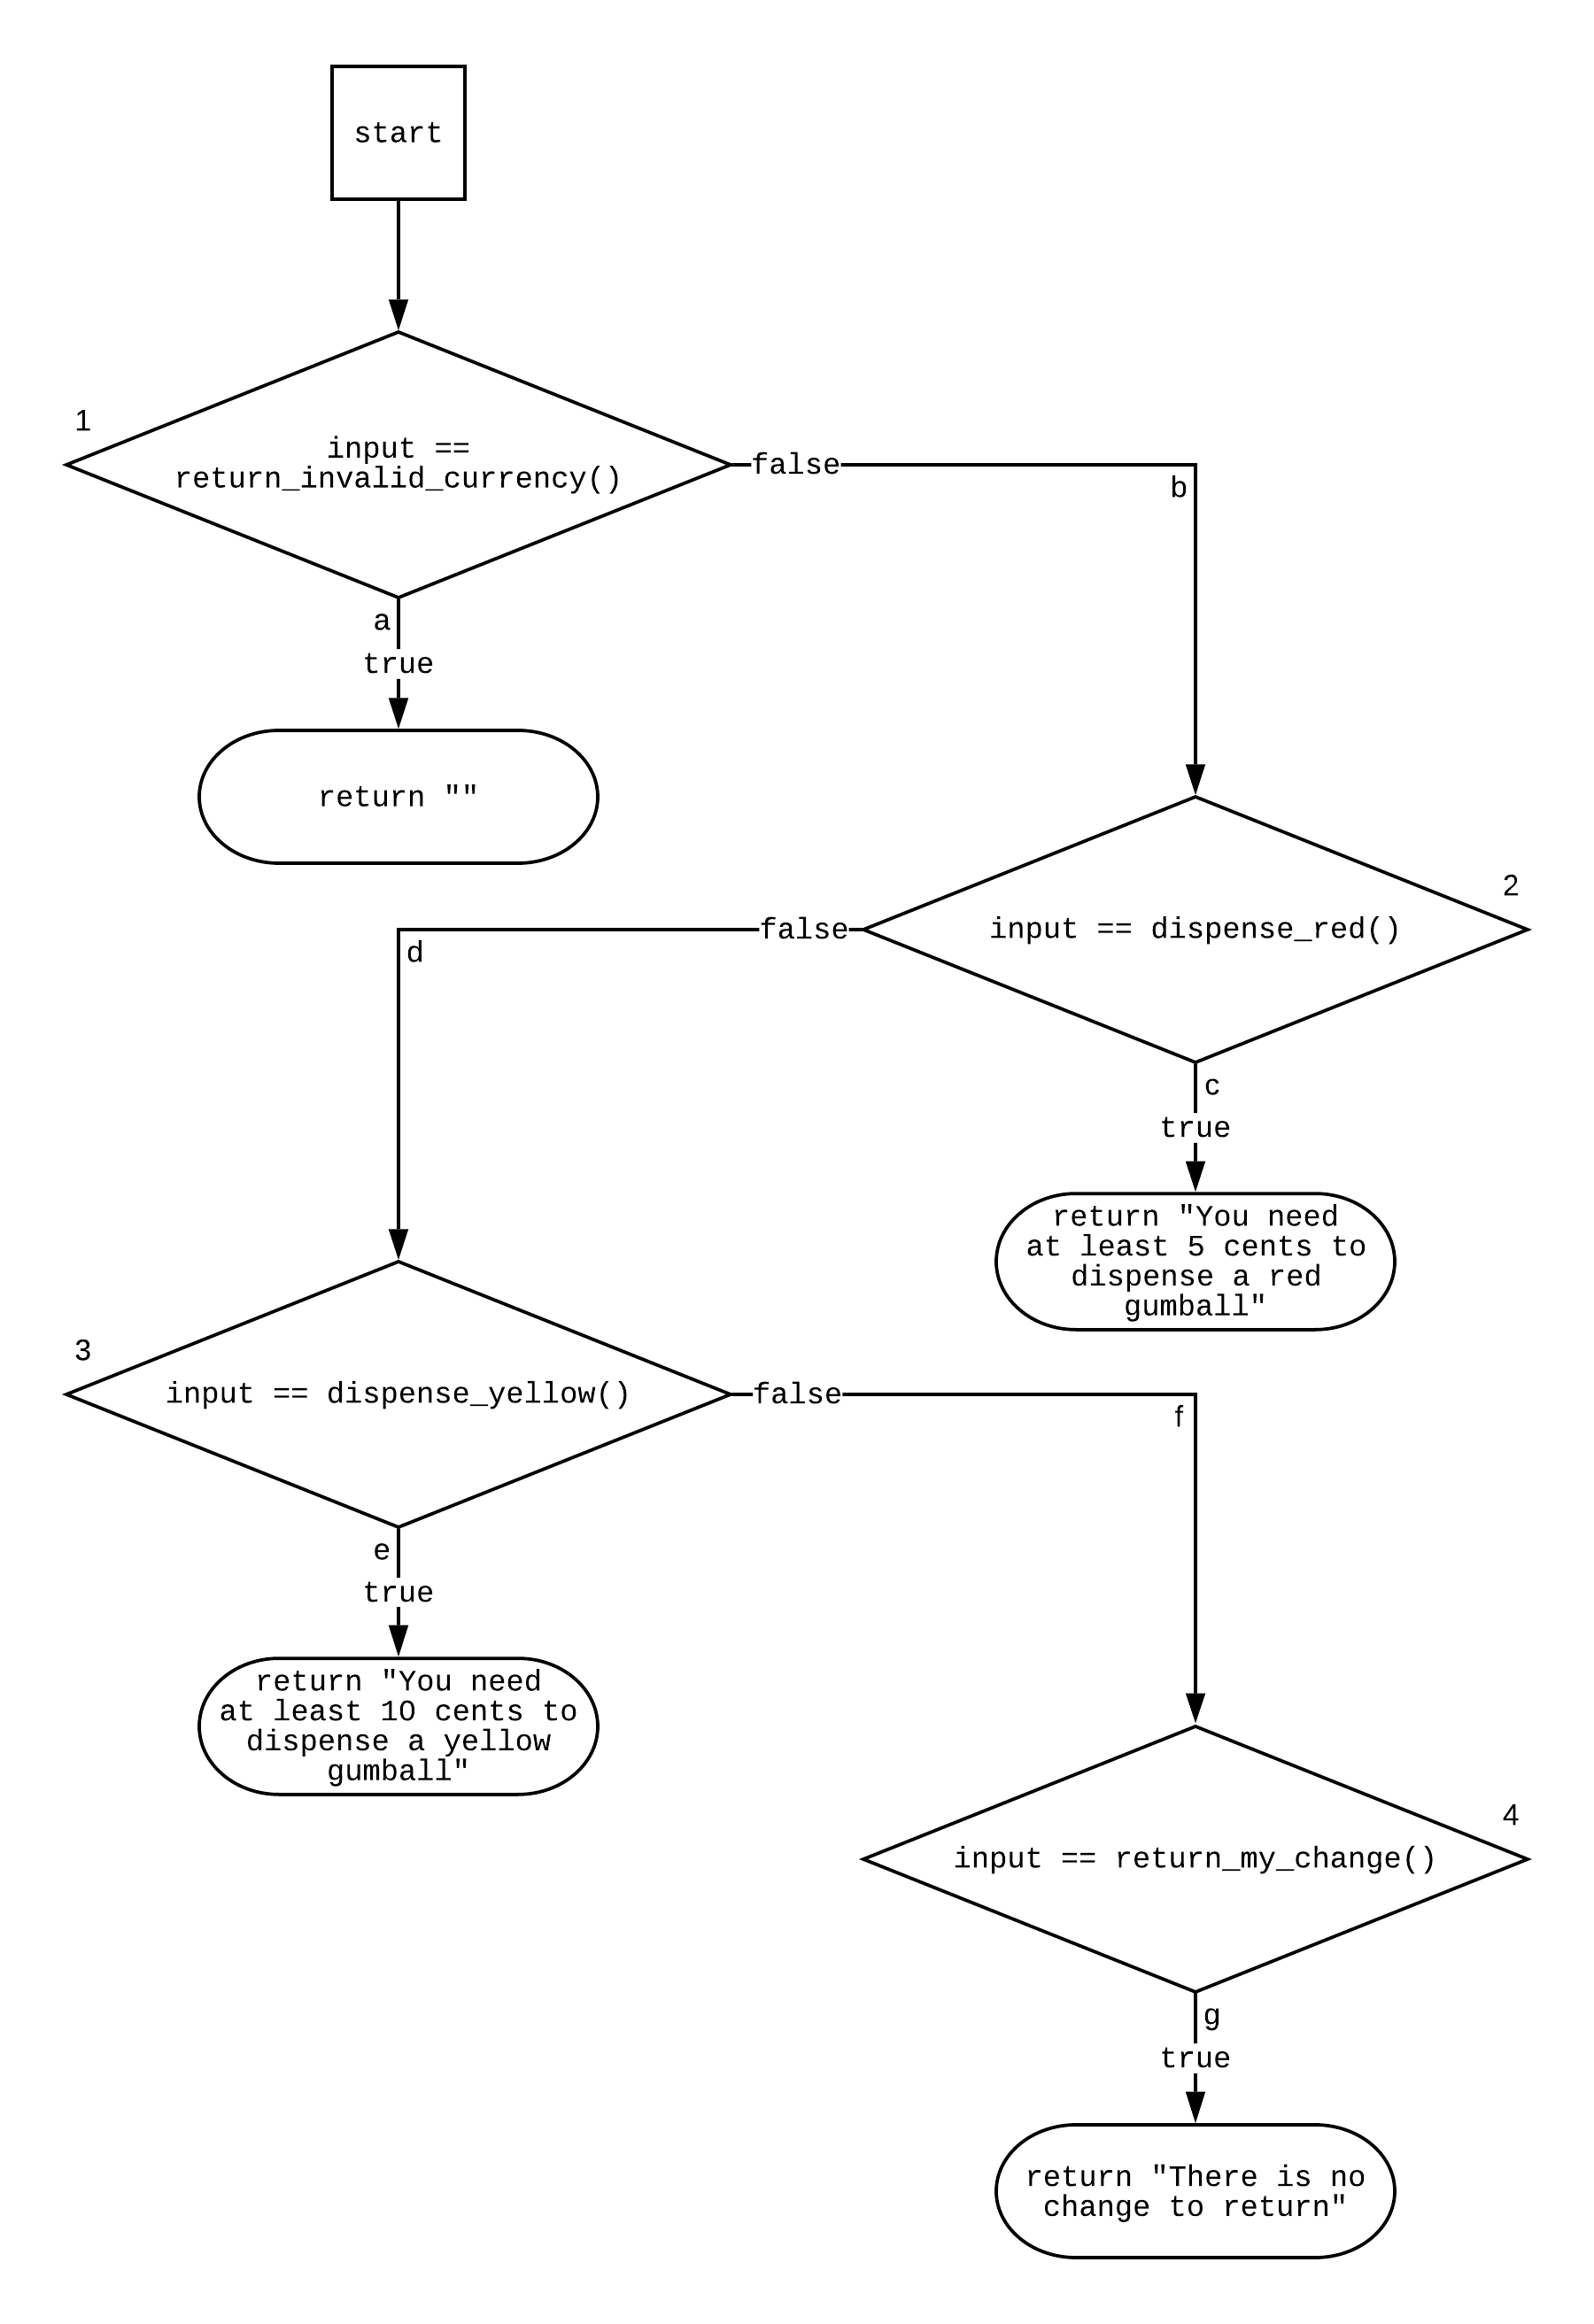
\includegraphics[width=12cm]{gumball-machine-control-flow.png}}
	\caption{Gumball Machine Control Flow Diagram (No Currency Inserted)}
\end{figure}
\pagebreak

Using the control flow diagram, we generate test cases to ensure statement coverage:
\begin{table}[!htb]
\centering
\begin{tabularx}{7cm}{llllllll}
\toprule
Path &
    a &
    b &
    c &
    d &
    e &
    f &
    g \\ \midrule
(a) &
    \checkmark &
    &
    &
    &
    &
    &
    \\ \midrule
(b, c) &
    &
    \checkmark &
    \checkmark &
    &
    &
    &
    \\ \midrule
(b, d, e) &
    &
    \checkmark &
    &
    \checkmark &
    \checkmark &
    &
    \\ \midrule 
(b, d, f, g) &
    &
    \checkmark &
    &
    \checkmark &
    &
    \checkmark &
    \checkmark \\ \bottomrule 
\end{tabularx}
\caption{Control Flow Testing Statement Coverage}
\end{table}

\begin{table}[!htb]
\begin{tabularx}{\textwidth}{lll}
\toprule
Path &
    Input Vector &
    Expected Output \\ \midrule
(a) &
    \texttt{<return\_invalid\_currency()>} &
    ``""\\ \midrule
(b, c) &
    \texttt{<dispense\_red()>} &
    ``You need at least 5 cents to dispense a red gumball"\\ \midrule
(b, d, e) &
    \texttt{<dispense\_yellow()>} &
    ``You need at least 10 cents to dispense a yellow gumball"\\ \midrule
(b, d, f, g) &
    \texttt{<return\_my\_change()>} &
    ``There is no change to return"\\ \bottomrule    
\end{tabularx}
\caption{Revised ``No Currency" Test Cases - Control Flow Testing}
\end{table}

\subsection{Equivalence Class Testing}
The input domain of ``all functions other than \texttt{insert()}" can be partitioned based on the remaining functions: 
\begin{itemize}
    \item{EC-01: \texttt{return\_invalid\_currency()}}
    \item{EC-02: \texttt{dispense\_red()}}
    \item{EC-03: \texttt{dispense\_yellow()}}
    \item{EC-04: \texttt{return\_my\_change()}}
\end{itemize}

We generate a test case for each uncovered equivalence class:
\begin{table}[!htb]
\begin{tabularx}{\textwidth}{cXXcccc}
\toprule
TC &
    Test Value &
    Expected Result &
    EC-01 &
    EC-02 &
    EC-03 &
    EC-04 \\ \midrule
01 &
    \texttt{<return\_invalid\_currency()>} &
    ``" &
    \checkmark &
    &
    & 
    \\ \midrule
02 &
    \texttt{<dispense\_red()>} &
    ``You need at least 5 cents to dispense a red gumball" &
    &
    \checkmark &
    & 
    \\ \midrule
03 &
    \texttt{<dispense\_yellow()>} &
    ``You need at least 10 cents to dispense a yellow gumball" &
    &
    &
    \checkmark & 
    \\ \midrule
04 &
    \texttt{<return\_my\_change()>} &
    ``There is no change to return" &
    &
    &
    &
    \checkmark \\ \bottomrule      
\end{tabularx}
\caption{Revised ``No Currency" Test Cases - Equivalence Class Testing}
\end{table}

%\section{Return Valid Currency Test Cases}
%\begin{table}[!htb]
%\begin{tabularx}{\textwidth}{XXX}
%\toprule
%Test Name &
%    Input Vector &
%    Expected Output \\ \midrule
%test return nickel &
%    \texttt{<insert("nickel"), return\_my\_change()>} &
%    ``Returning your change of 5 cents" \\ \midrule
%test return dime &
%    \texttt{<insert("dime"), return\_my\_change()>} &
%    ``Returning your change of 10 cents" \\ \midrule
%test return quarter &
%    \texttt{<insert("quarter"), return\_my\_change()>} &
%    ``Returning your change of 25 cents" \\ \bottomrule
%\end{tabularx}
%\end{table}

\newpage
\section{Exact Currency Test Cases - Original Test Cases}
\begin{table}[!htb]
\begin{tabularx}{\textwidth}{XXX}
\toprule
Test Name &
    Input Vector &
    Expected Output \\ \midrule
test insert nickel dispense red &
    \texttt{<insert("nickel"), dispense\_red()} &
    ``Enjoy your red gumball" \\ \midrule
test insert dime dispense yellow &
    \texttt{<insert("nickel"), dispense\_yellow()>} &
    ``Enjoy your yellow gumball" \\ \midrule
test insert nickels dispense yellow &
    \texttt{<insert("nickel"), insert("nickel"), dispense\_yellow()>} &
    ``Enjoy your yellow gumball" \\ \bottomrule
\end{tabularx}
\caption{Original "Exact Currency" Test Cases}
\end{table}

Of these three test cases, no particular technique (e.g. control flow testing, data flow testing, etc.) was used in their creation.

\newpage
\section{Exact Currency Test Cases - Revised Test Cases}
In general, we assume the gumball machine has enough currency when applicable.

\subsection{Conformance Testing}
\begin{figure}[h!]
	\centerline{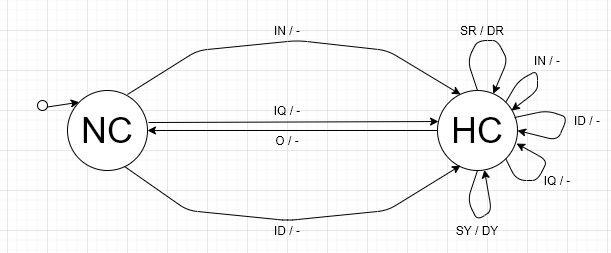
\includegraphics[width=\textwidth]{gumball-machine-finite-state-machine.png}}
	\caption{FSM Model of Gumball Machine (Exact Currency Subset)}
\end{figure}

\begin{table}[htb!]
\centering
\begin{tabularx}{11cm}{lll}
\toprule
Abbreviation &
    Expanded Form &
    Meaning \\ \midrule
NC &
    No currency &
    The machine has no currency \\ \midrule
HC &
    Has currency &
    The machine has some currency \\ \bottomrule
\end{tabularx}
\caption{Set of States in FSM of Figure 2}
\end{table}

\begin{table}[htb!]
\centering
\begin{tabularx}{9.25cm}{ll}
\toprule
Inputs &
    Outputs \\ \midrule
IN: Insert nickel &
    DR: Dispense red gumball \\ \midrule
ID: Insert dime &
    DY: Dispense yellow gumball \\ \midrule
IQ: Insert quarter &
    ---: No output \\ \midrule
SR: Select red gumball &
    \\ \midrule
SY: Select yellow gumball &
    \\ \midrule
O: Out of currency &
    \\ \bottomrule
\end{tabularx}
\caption{Input and Output Sets in FSM of Figure 2}
\end{table}

\pagebreak
\begin{table}[htb!]
\centering
\begin{tabularx}{13cm}{lp{5cm}p{6cm}}
\toprule
Test Case &
    Test Sequence &
    Expected Output \\ \midrule
1 &
    \begin{itemize}
        \item{$<$NC, IN / ---, HC$>$}
        \item{$<$HC, SR / DR, HC$>$}
        \item{$<$HC, O / ---, NC$>$}
    \end{itemize} &
    ``Enjoy your red gumball" \\ \midrule
2 &
    \begin{itemize}
        \item{$<$NC, ID / ---, HC$>$}
        \item{$<$HC, SY / DY, HC$>$}
        \item{$<$HC, O / ---, NC$>$}
    \end{itemize} &
    ``Enjoy your yellow gumball" \\ \midrule
3 &
    \begin{itemize}
        \item{$<$NC, IN / ---, HC$>$}
        \item{$<$HC, IN / ---, HC$>$}
        \item{$<$HC, SY / DY, HC$>$}
        \item{$<$HC, O / ---, NC$>$}
    \end{itemize} &
    ``Enjoy your yellow gumball" \\ \midrule
4 &
    \begin{itemize}
        \item{$<$NC, IQ / ---, HC$>$}
        \item{$<$HC, SY / DY, HC$>$}
        \item{$<$HC, SR / DR, HC$>$}
        \item{$<$HC, SY / DY, HC$>$}
        \item{$<$HC, O / ---, NC$>$}
    \end{itemize} &
    \begin{itemize}
        \item{``Enjoy your yellow gumball"}
        \item{``Enjoy your red gumball"}
        \item{``Enjoy your yellow gumball"}
    \end{itemize} \\ \bottomrule
\end{tabularx}
\caption{Revised ``Exact Currency" Test Cases - Conformance Testing}
\end{table}

\pagebreak
%\section{Invalid Currency Test Cases}
%\begin{table}[!htb]
%\begin{tabularx}{\textwidth}{XXX}
%\toprule
%Test Name &
%    Input Vector &
%    Expected Output \\ \midrule
%test return dollar &
%    \texttt{<insert("dollar"), return\_my\_change()>} &
%    ``Returning your invalid currency of dollar" \\ \midrule
%test return dollars &
%    \texttt{<insert("dollar"), insert("dollar"), return\_my\_change()>} &
%    ``Returning your invalid currency of dollar, dollar" \\ \midrule
%test insert dollar dispense red &
%    \texttt{<insert("dollar"), dispense\_red()>} &
%    ``Returning your invalid currency of dollar" \\ \midrule
%test insert dollar dispense yellow &
%    \texttt{<insert("dollar"), dispense\_yellow()>} &
%    ``Returning your invalid currency of dollar" \\ \bottomrule
%\end{tabularx}
%\end{table}
%
%\section{Multiple Gumballs Exact Currency Test Cases}
%\begin{table}[!htb]
%\begin{tabularx}{\textwidth}{XXX}
%\toprule
%Test Name &
%    Input Vector &
%    Expected Output \\ \midrule
%test insert nickels dispense reds &
%    \texttt{<insert("nickel"), insert("nickel"), dispense\_red(), dispense\_red(), return\_my\_change()>} &
%    ``There is no change to return" \\ \midrule
%test insert dime dispense reds &
%    \texttt{<insert("dime"), dispense\_red(), dispense\_red(), return\_my\_change()>} &
%    ``There is no change to return" \\ \midrule
%test insert nickels dispense yellows &
%    \texttt{<insert("nickel"), insert("nickel"), insert("nickel"), insert("nickel"), dispense\_yellow(), dispense\_yellow(), return\_my\_change()>} &
%    ``There is no change to return" \\ \midrule
%test insert dimes dispense yellows &
%    \texttt{<insert("dime"), insert("dime"), dispense\_yellow(), dispense\_yellow(), return\_my\_change()>} &
%    ``There is no change to return" \\ \bottomrule
%\end{tabularx}
%\end{table}

\end{document}